\subsection{$n$ 重积分}

\begin{example}
    Volume of $n$-simplex: $\Delta_n(a)=\left\{(x_1,\dots,x_n)\in\mathbb{R}^n\middle|x_1,\dots, x_n\geq 0,\ x_1+\dots+x_n\leq a\right\}$

    \begin{align*}
        \sigma\left(\Delta_n(a)\right)
         & =\int_{\Delta_n(a)}\,\mathrm{d}\sigma                                      \\
         & =\int_{\substack{x_1,\dots, x_n\geq 0                                      \\
        x_1+\dots+x_n\leq a}}\,\mathrm{d}x_1\cdots\mathrm{d}x_n                       \\
         & \xlongequal{x_i=ay_i}a^n\int_{\substack{y_1,\dots, y_n\geq 0               \\
        y_1+\dots+y_n\leq 1}}\,\mathrm{d}y_1\cdots\mathrm{d}y_n                       \\
         & =a^n\int_0^1\,\mathrm{d}y_n\int_{\substack{y_1,\dots, y_{n-1}\geq 0        \\
        y_1+\dots+y_{n-1}\leq 1-y_n}}\,\mathrm{d}y_1\cdots\mathrm{d}y_{n-1}           \\
         & =a^n\int_0^1(1-y_n)^{n-1}\sigma\left(\Delta_{n-1}(1)\right)\,\mathrm{d}y_n \\
         & =a^n\sigma\left(\Delta_{n-1}(1)\right)\frac{1}{n}
    \end{align*}

    $\sigma(\Delta_n(1))=\frac{1}{n}\sigma(\Delta_{n-1}(1))=\dots=\frac{1}{n!}\sigma(\Delta_1(1))=\frac{1}{n!}$

    $\boxed{\sigma_n(a)=\frac{a^n}{n!}}$
\end{example}

\begin{example}
    $B_n(a)=\left\{(x_1,\dots,x_n)\in\mathbb{R}^n\middle|x_1^2+\dots+x_n^2\leq a^2\right\}$

    $\sigma(B_n(a))=\int_{x_1^2+\dots+x_n^2\leq a^2}\,\mathrm{d}x_1\cdots\mathrm{d}x_n=a^n\cdot\sigma(B_n(1))$

    \begin{center}
        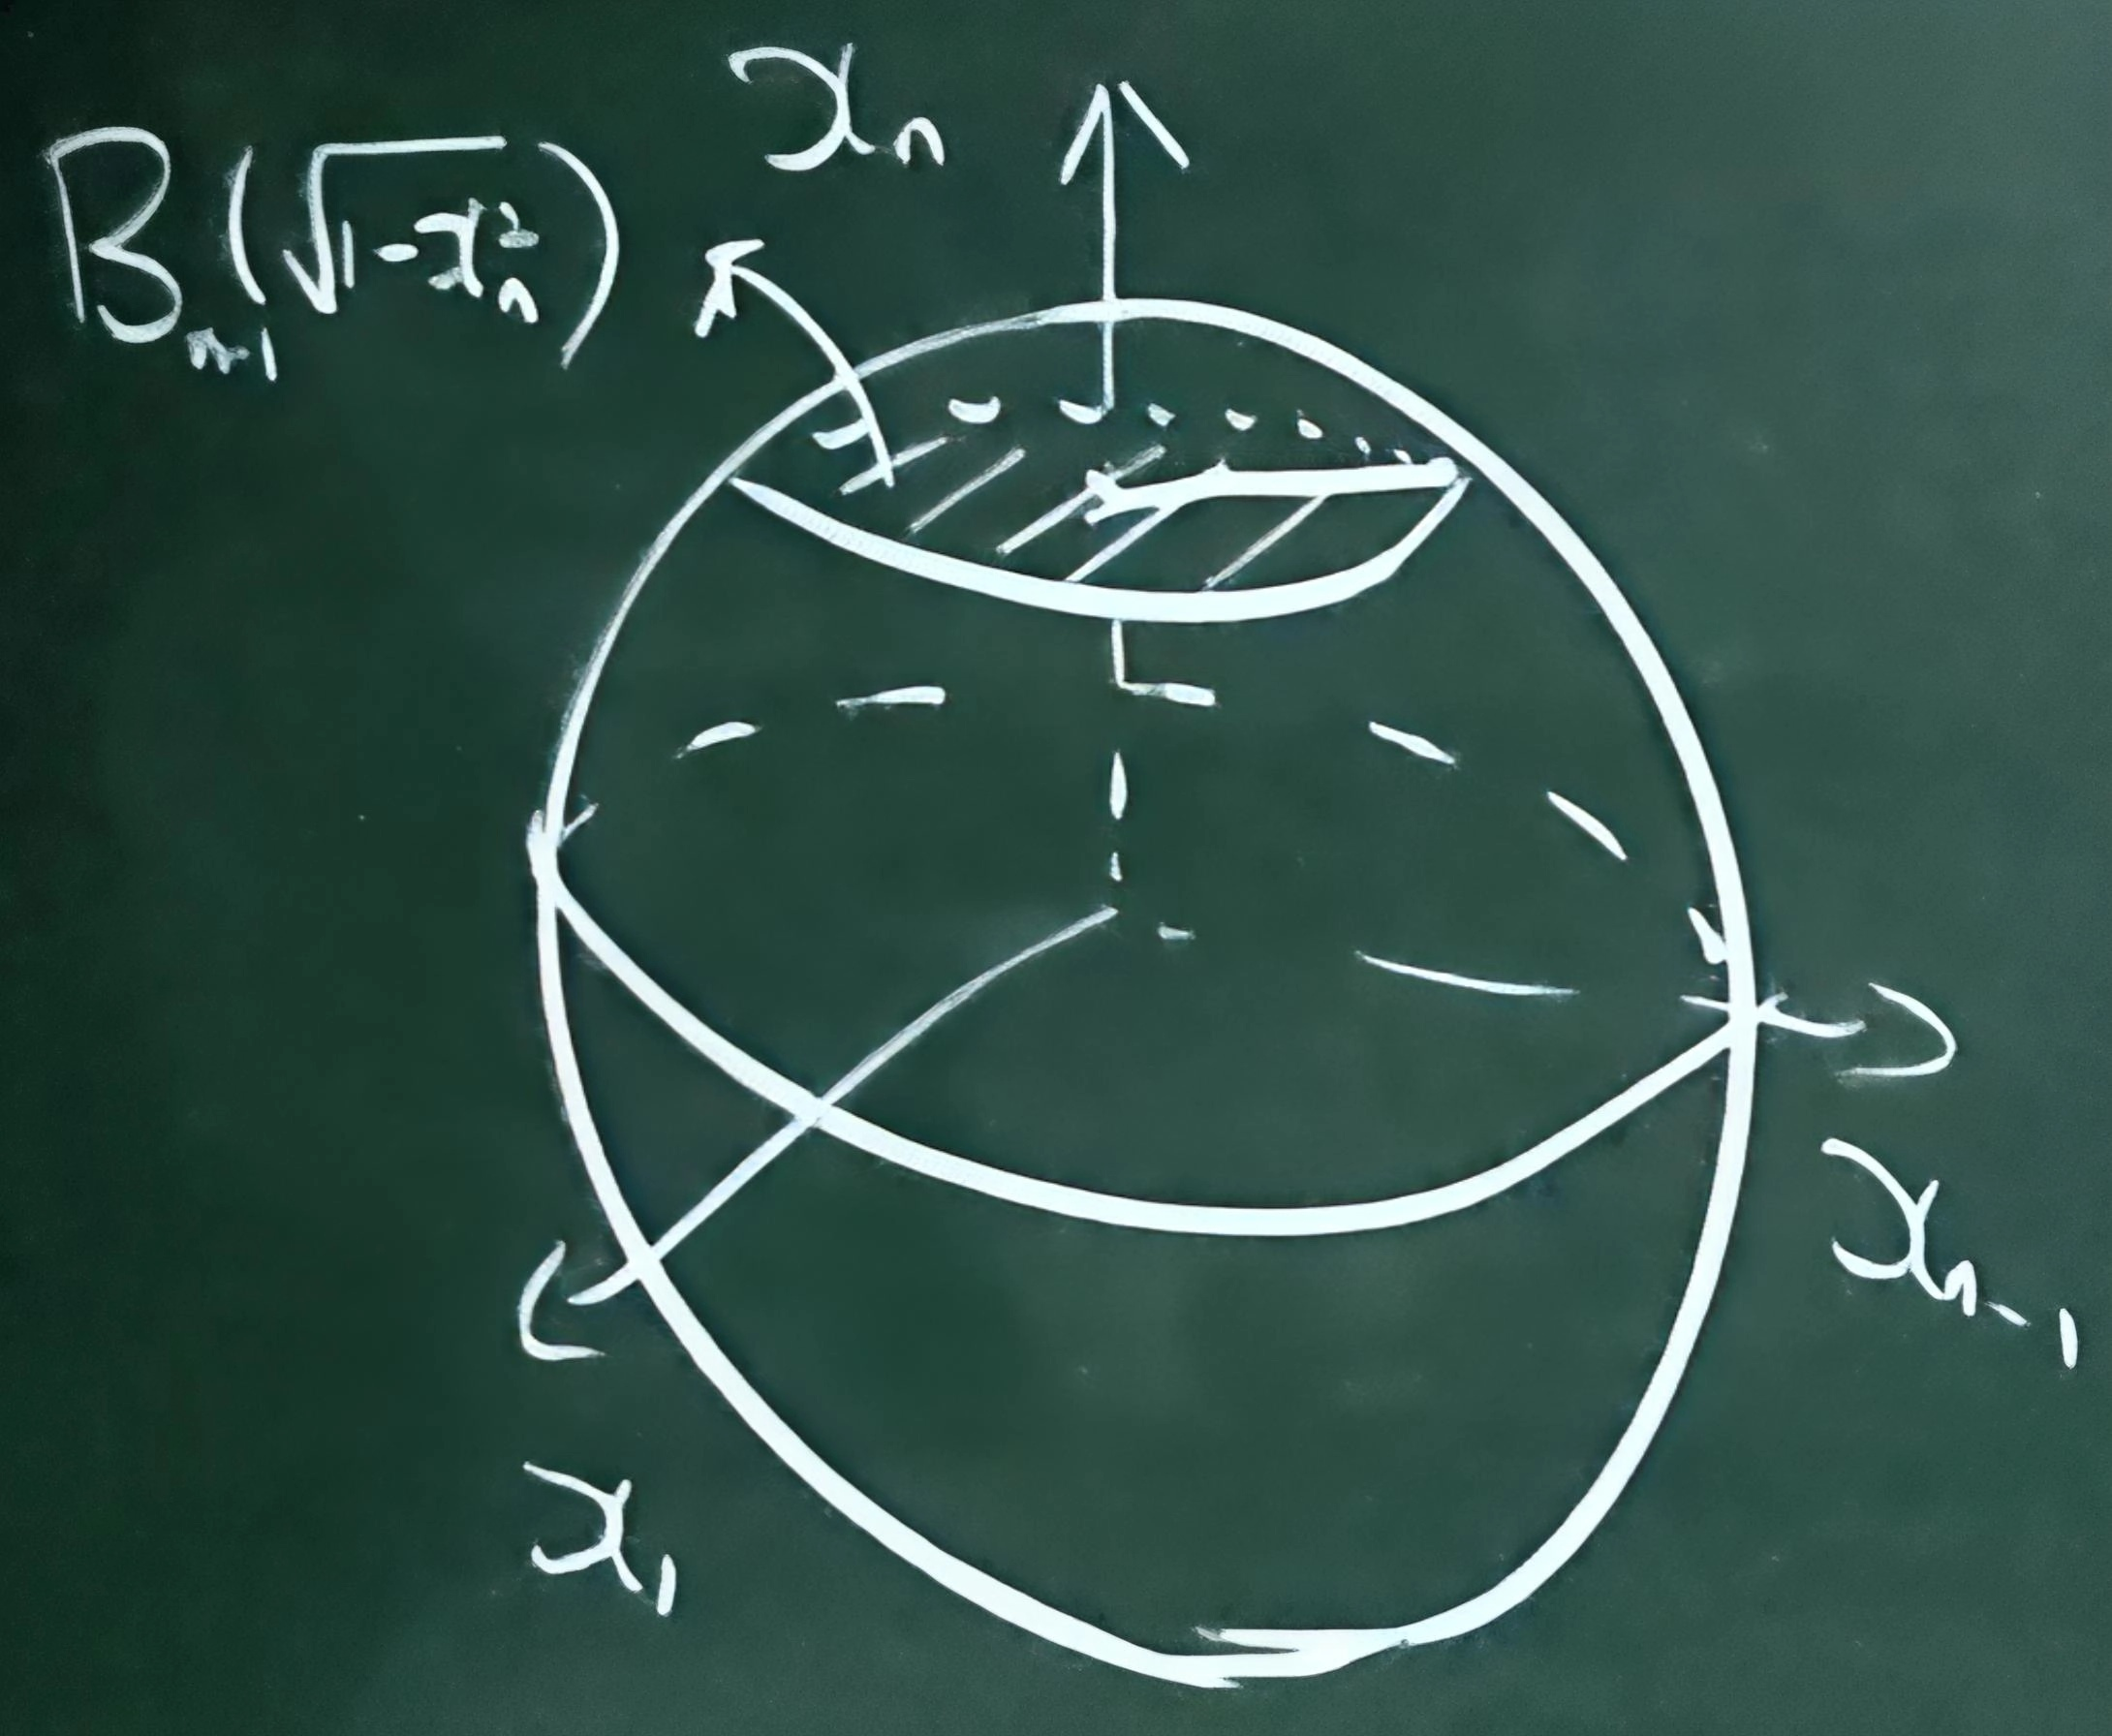
\includegraphics[height=2cm]{chapters/10/04/01}
    \end{center}

    \begin{align*}
        \sigma(B_n(1))
         & =\int_{-1}^1\,\mathrm{d}x_n\int_{x_1^2+\dots+x_{n-1}^2\leq 1-x_n^2}\,\mathrm{d}x_1\cdots\mathrm{d}x_{n-1}                                                    \\
         & =\int_{-1}^1(1-x_n^2)^{\frac{n-1}{2}}\,\mathrm{d}x_n\cdot\sigma(B_{n-1}(1))                                                                                  \\
         & \xlongequal[\mathrm{d}x_n=\cos\theta\,\mathrm{d}\theta]{x_n=\sin\theta}\sigma(B_{n-1}(1))\int_{-\frac{\pi}{2}}^{\frac{\pi}{2}}\cos^n\theta\,\mathrm{d}\theta \\
    \end{align*}

    \begin{align*}
        \sigma(B_n(1))
         & =\iint_{u^2+v^2\leq 1}\,\mathrm{d}u\mathrm{d}v\int_{x_1^2+\dots+x_{n-2}^2\leq 1-u^2-v^2}\,\mathrm{d}x_1\cdots\mathrm{d}x_{n-2} \\
         & =\iint_{u^2+v^2\leq 1}(1-u^2-v^2)^{\frac{n-2}{2}}\,\mathrm{d}u\mathrm{d}v\cdot\sigma(B_{n-2}(1))                               \\
         & =\int_0^1\int_0^{2\pi}(1-r^2)^{\frac{n-2}{2}}r\,\mathrm{d}\theta\mathrm{d}r\cdot\sigma(B_{n-2}(1))                             \\
         & =2\pi\left(\left.-\frac{1}{n}(1-r^2)^{\frac{n}{2}}\right|_0^1\right)\sigma(B_{n-2}(1))                                         \\
         & =\frac{2\pi}{n}\sigma(B_{n-2}(1))
    \end{align*}

    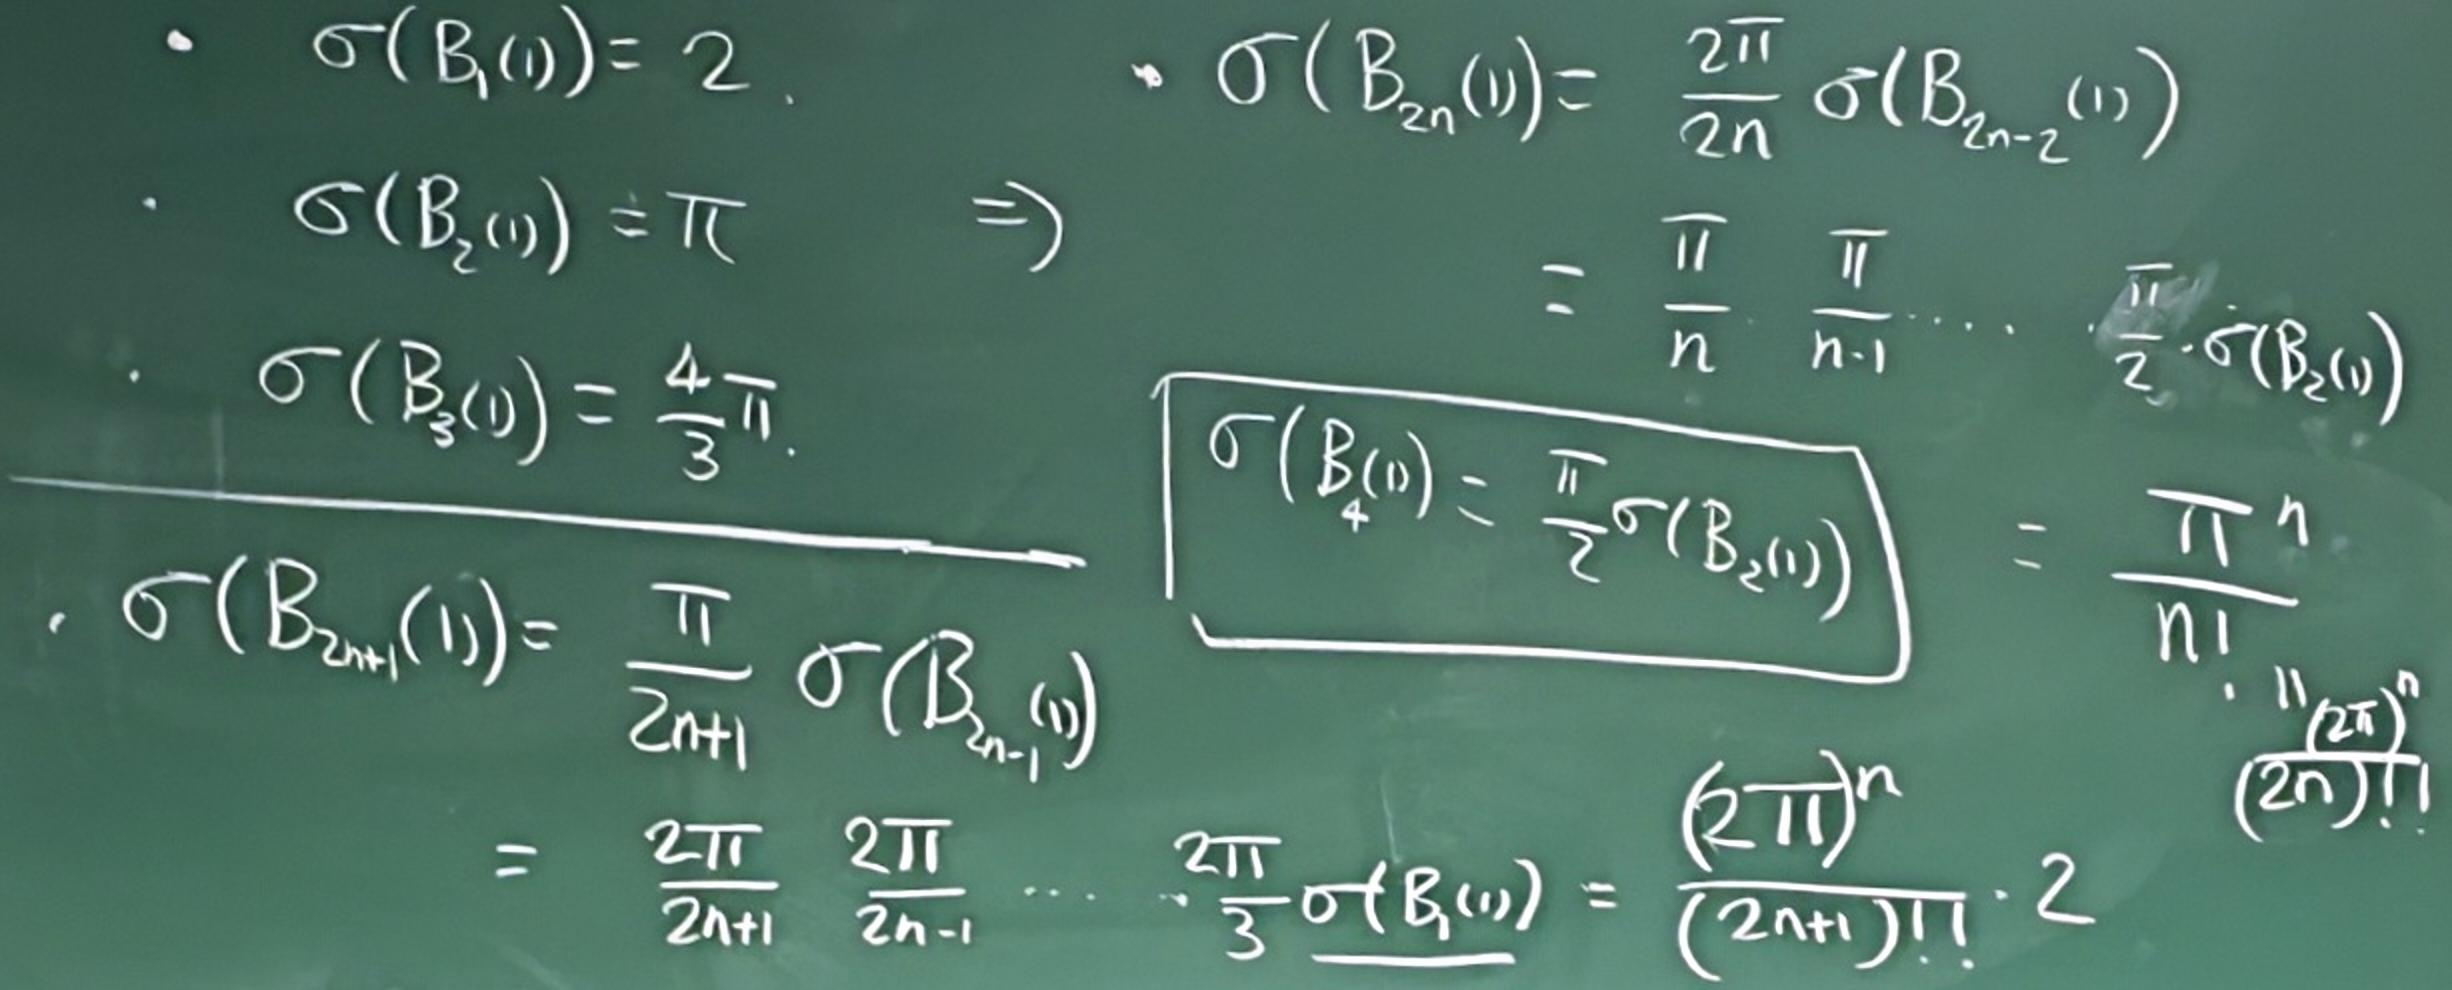
\includegraphics[height=5cm]{chapters/10/04/02}
\end{example}